%%%%%%%%%%%%%%%%%%%%%%%%%%%%%%%%%%%%%%%%%%%%%%%%%%%%%%%%%%
\frame {\frametitle{What is Apache Spark}
%%%%%%%%%%%%%%%%%%%%%%%%%%%%%%%%%%%%%%%%%%%%%%%%%%%%%%%%%%
\begin{itemize}
  \item {\bf Project goals}
  \begin{itemize}
    \item Generality: diverse workloads, operators, job sizes
    \item Low latency: sub-second
    \item Fault tolerance: faults are the norm, not the exception
    \item Simplicity: often comes from generality
  \end{itemize}
\end{itemize}

}

%%%%%%%%%%%%%%%%%%%%%%%%%%%%%%%%%%%%%%%%%%%%%%%%%%%%%%%%%%
\frame {\frametitle{Motivations}
%%%%%%%%%%%%%%%%%%%%%%%%%%%%%%%%%%%%%%%%%%%%%%%%%%%%%%%%%%
\begin{itemize}
  \item {\bf Software engineering point of view}
  \begin{itemize}
    \item Hadoop code base is huge
    \item Contributions/Extensions to Hadoop are cumbersome
    \item Java-only hinders wide adoption, but Java support is fundamental
  \end{itemize}

\vspace{20pt}

  \item {\bf System/Framework point of view}
  \begin{itemize}
    \item Unified pipeline
    \item Simplified data flow
    \item Faster processing speed
  \end{itemize}

\vspace{20pt}

  \item {\bf Data abstraction point of view}
  \begin{itemize}
    \item New fundamental abstraction RDD
    \item Easy to extend with new operators
    \item More descriptive computing model
  \end{itemize}
\end{itemize}
}

%%%%%%%%%%%%%%%%%%%%%%%%%%%%%%%%%%%%%%%%%%%%%%%%%%%%%%%%%%
\frame {\frametitle{Hadoop: No Unified Vision}
%%%%%%%%%%%%%%%%%%%%%%%%%%%%%%%%%%%%%%%%%%%%%%%%%%%%%%%%%%
\begin{figure}[h]
  \centering
  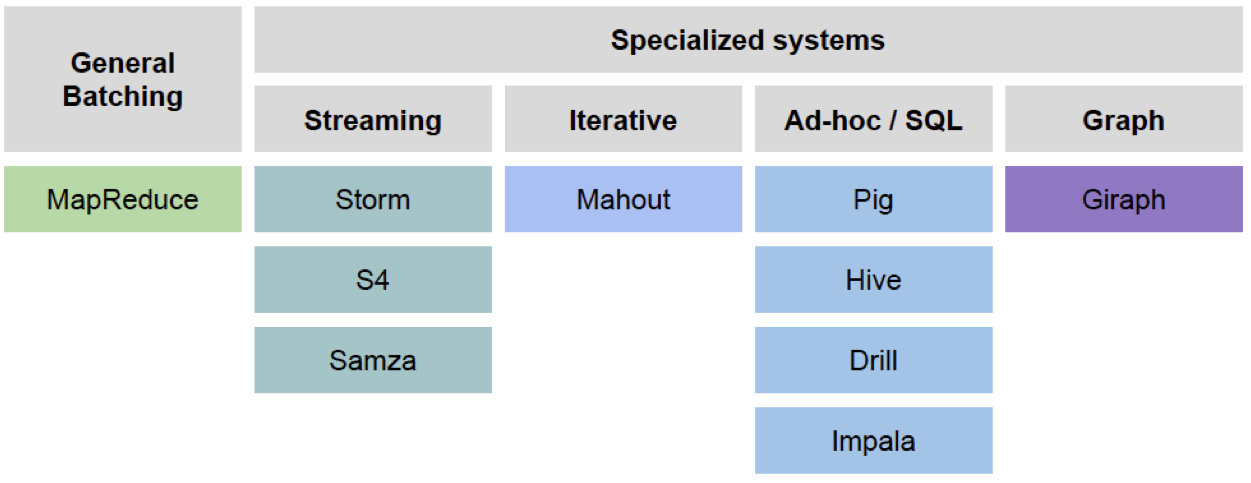
\includegraphics[scale=0.25]{./Figures/hadoop_modules}
  \label{fig:spark_modules}
\end{figure}
\begin{itemize}
    \item Sparse modules
    \item Diversity of APIs
    \item Higher operational costs
\end{itemize}
}

%%%%%%%%%%%%%%%%%%%%%%%%%%%%%%%%%%%%%%%%%%%%%%%%%%%%%%%%%%
\frame {\frametitle{SPARK: A Unified Pipeline}
%%%%%%%%%%%%%%%%%%%%%%%%%%%%%%%%%%%%%%%%%%%%%%%%%%%%%%%%%%
\begin{figure}[h]
  \centering
  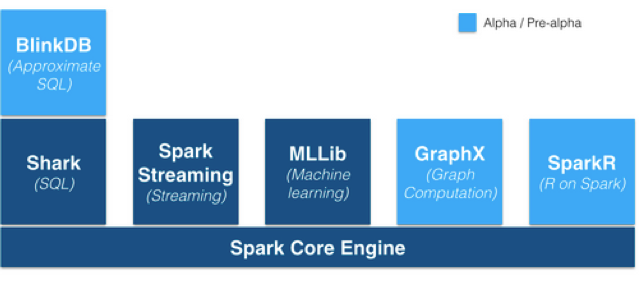
\includegraphics[scale=0.4]{./Figures/spark_modules}
  \label{fig:spark_modules}
\end{figure}
\begin{itemize}
    \item Spark Streaming (stream processing)
    \item GraphX (graph processing)
    \item MLLib (machine learning library)
    \item Spark SQL (SQL on Spark) 
\end{itemize}
}

%%%%%%%%%%%%%%%%%%%%%%%%%%%%%%%%%%%%%%%%%%%%%%%%%%%%%%%%%%
\frame {\frametitle{A Simplified Data Flow}
%%%%%%%%%%%%%%%%%%%%%%%%%%%%%%%%%%%%%%%%%%%%%%%%%%%%%%%%%%
\begin{figure}[h]
  \centering
  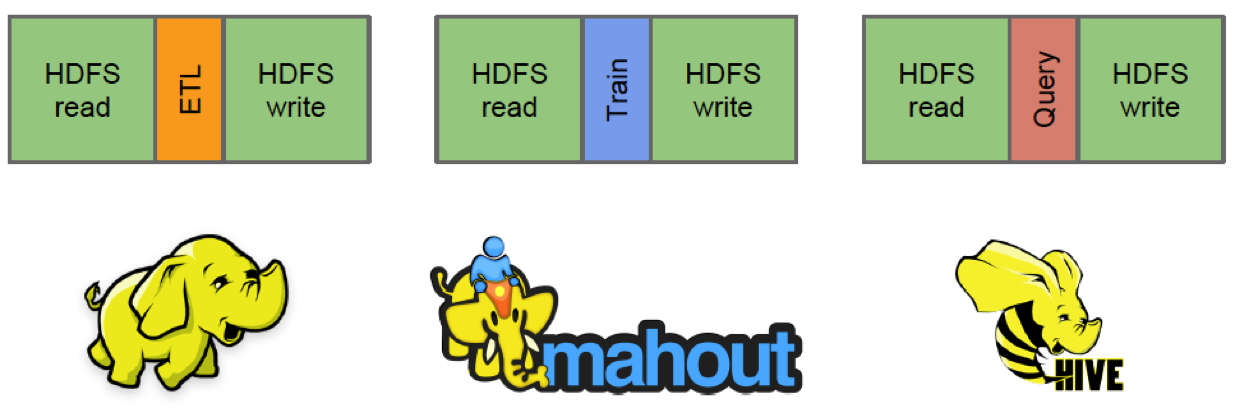
\includegraphics[scale=0.25]{./Figures/data_flow_hadoop}
  \label{fig:data_flow_hadoop}
\end{figure}

\begin{figure}[h]
  \centering
  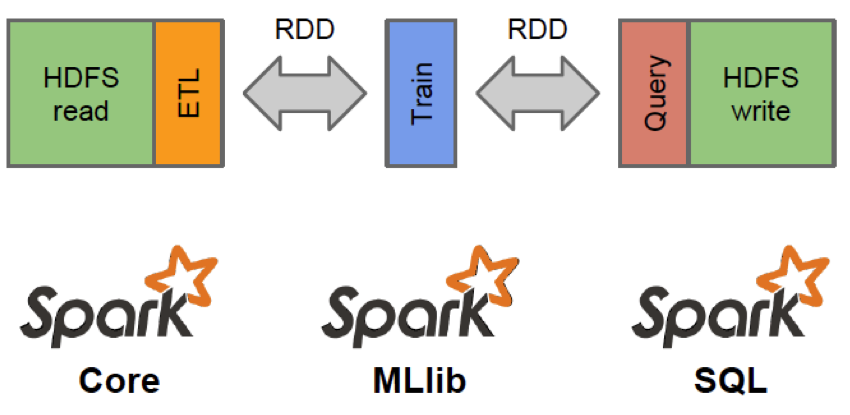
\includegraphics[scale=0.25]{./Figures/data_flow_spark}
  \label{fig:data_flow_spark}
\end{figure}
}

%%%%%%%%%%%%%%%%%%%%%%%%%%%%%%%%%%%%%%%%%%%%%%%%%%%%%%%%%%
\frame {\frametitle{Hadoop: Bloated Computing Model}
%%%%%%%%%%%%%%%%%%%%%%%%%%%%%%%%%%%%%%%%%%%%%%%%%%%%%%%%%%
\begin{figure}[h]
  \centering
  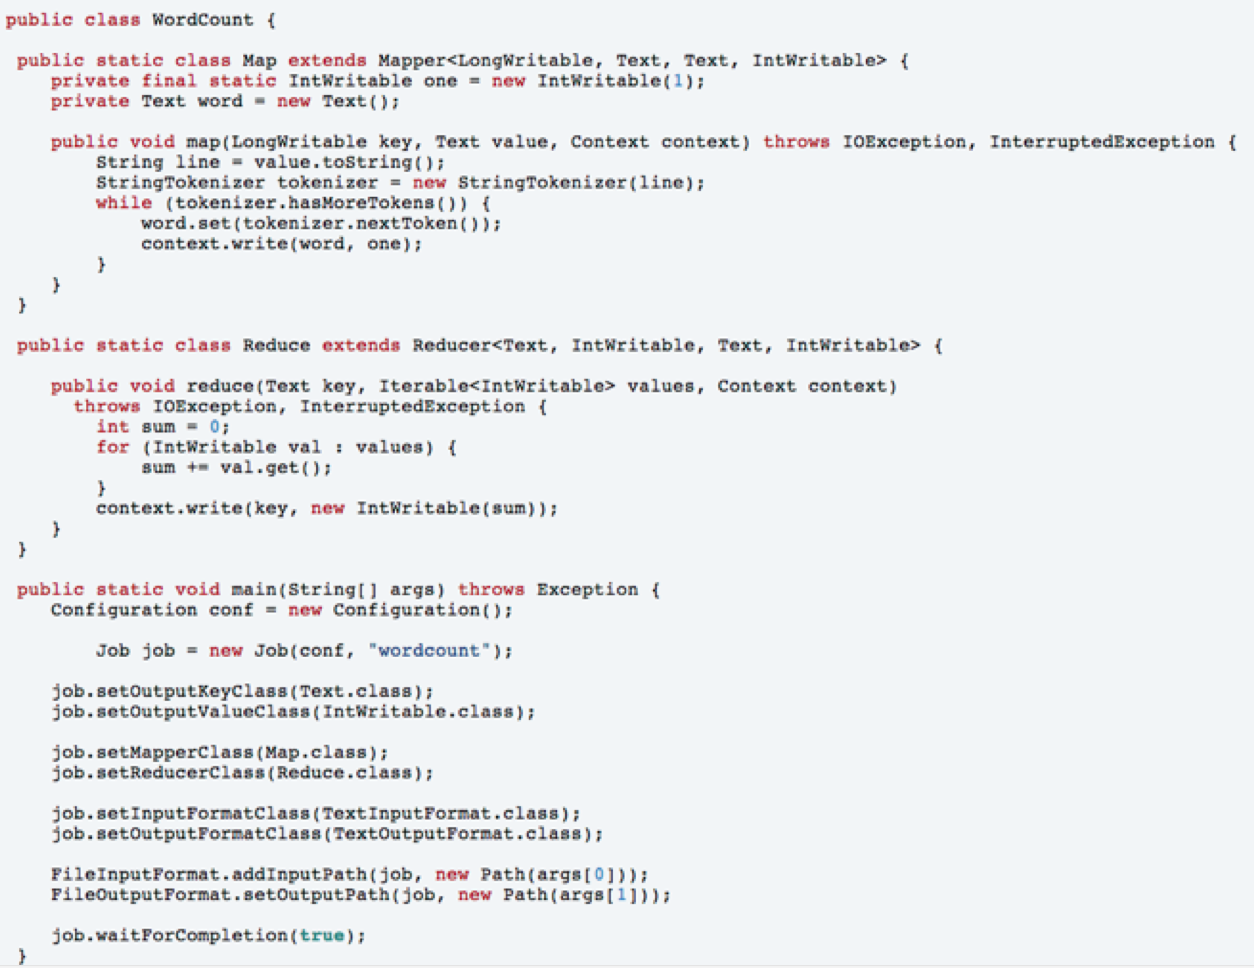
\includegraphics[scale=0.2]{./Figures/wc_hadoop}
  \label{fig:wc_hadoop}
\end{figure}
}

%%%%%%%%%%%%%%%%%%%%%%%%%%%%%%%%%%%%%%%%%%%%%%%%%%%%%%%%%%
\begin{frame}[fragile]
\frametitle{SPARK: Descriptive Computing Model}
%%%%%%%%%%%%%%%%%%%%%%%%%%%%%%%%%%%%%%%%%%%%%%%%%%%%%%%%%%
% \begin{figure}[h]
%   \centering
%   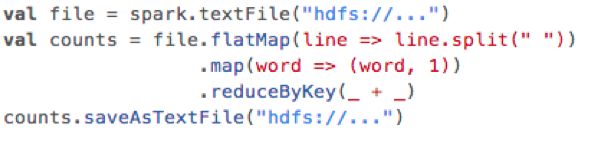
\includegraphics[scale=0.36]{./Figures/wc_spark}
%   \label{fig:wc_spark}
% \end{figure}

\begin{lstlisting}
val file = sc.textFile("hdfs://...")

val counts = file.flatMap(line => line.split(" "))
    .map(word => (word,1))
    .reduceByKey(_ + _)

counts.saveAsTextFile("hdfs://...")
\end{lstlisting}


\begin{itemize}
  \item Organize computation into multiple stages in a processing pipeline
  \begin{itemize}
    \item \textbf{Transformations} apply user code to distributed data in parallel
   \item \textbf{Actions} assemble final output of an algorithm, from distributed data
  \end{itemize}
    
  \end{itemize}  
\end{frame}

%%%%%%%%%%%%%%%%%%%%%%%%%%%%%%%%%%%%%%%%%%%%%%%%%%%%%%%%%%
\frame {\frametitle{Faster Processing Speed}
%%%%%%%%%%%%%%%%%%%%%%%%%%%%%%%%%%%%%%%%%%%%%%%%%%%%%%%%%%
\begin{itemize}
  \item {\bf Let's focus on iterative algorithms}
  \begin{itemize}
    \item Spark is faster thanks to the simplified data flow
    \item We avoid materializing data on HDFS after each iteration
  \end{itemize}

\vspace{20pt}

  \item {\bf Example: k-means algorithm, 1 iteration}
  \begin{itemize}
    \item \texttt{HDFS Read}
    \item \textbf{\texttt{Map}}(\emph{Assign sample to closest centroid})
    \item \textbf{\texttt{GroupBy}}(Centroid\_ID)
    \item \texttt{NETWORK Shuffle}
    \item \textbf{\texttt{Reduce}}(\emph{Compute new centroids})
    \item \texttt{HDFS Write}
  \end{itemize}
  % \begin{itemize}
  %   \item Step 1: Place randomly initial group centroids into the space
  %   \item Step 2: Assign each object to the group that has the closest centroid.
  %   \item Step 3: Recalculate the positions of the centroids.
  %   \item Step 4: If the positions of the centroids didn't change go to the next step, else go to Step 2.
  %   \item Step 5: End.
  % \end{itemize}
\end{itemize}
}

%%%%%%%%%%%%%%%%%%%%%%%%%%%%%%%%%%%%%%%%%%%%%%%%%%%%%%%%%%
\frame {\frametitle{Code Base (2012)}
%%%%%%%%%%%%%%%%%%%%%%%%%%%%%%%%%%%%%%%%%%%%%%%%%%%%%%%%%%
\begin{figure}[h]
  \centering
  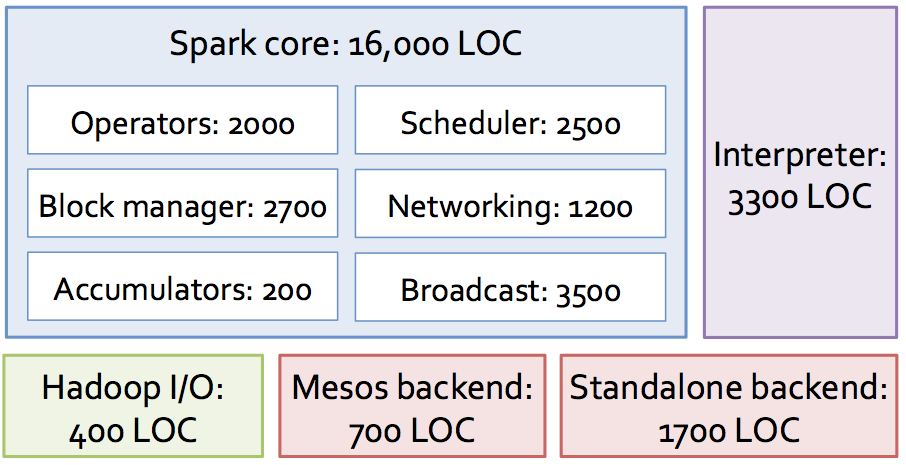
\includegraphics[scale=0.36]{./Figures/code_base}
  % \caption{Spark code base, as of 0.6.x (2012).}
  \label{fig:code_base}
\end{figure}

\begin{itemize}
  \item 2012 (version 0.6.x): 20,000 lines of code
  \item 2014 (branch-1.0): 50,000 lines of code
\end{itemize}
}
